\documentclass[12pt]{article}
\usepackage[usenames]{color} %used for font color
\usepackage{amssymb} %maths
\usepackage{amsmath} %maths
\usepackage[utf8]{inputenc} %useful to type directly diacritic characters
\usepackage[T1]{fontenc}
\usepackage{polski}

% \usepackage{listings}
\usepackage[theme=default-plain]{jlcode} % https://github.com/wg030/jlcode
\usepackage{graphicx}  %grafika

%\usepackage{subcaption} %dwa rysunki obok siebie
%\graphicspath{ {./rysunki/} } %skąd ma pobierać grafikę
%\usepackage{svg} % for graphics in svg, with the first compilation enable: "-shell-escape" to use tools to convert svg
%\usepackage{csvsimple} % to insert csv files 

\usepackage[a4paper, left=3cm, right=3cm, top=1.5cm, bottom=2cm]{geometry}


\setlength{\parskip}{10pt}
\setlength{\parindent}{0pt}

\title{Oscylator Van der Polla}
\author{Bartosz Zbik}
\date{2024-04-28} %format jest dowolny(może być nawet miesiąc słownie

\begin{document}
\maketitle %tworzy tytuł dokumentu

Jawnie zamieniłem równanie drugiego stopnia
\begin{equation}
\ddot x = - x  - \mu (x^2 - 1) \dot x
\end{equation}
na układ dwóch równań stopnia pierwszego
\begin{equation}
\begin{cases}
\dot x = v \\
\dot v  =  - x  - \mu (x^2 - 1) v
\end{cases}.
\end{equation}

Przedstawiony poniżej kod głównie służy do generowania rysunków, a cała logika rozwiązania równania znajduje się w definicji
\texttt{vanderpol!} oraz \texttt{findsol}.

Rozważyłem również przypadek $\mu=0$ nie wymieniony w poleceniu, żeby zobaczyć, że problem redukuje się do oscylatora harmonicznego.

\section{Kod}
\jlinputlisting{solution.jl}
\clearpage


\section{Wizualizacja wyników}

%
%
% plots for mu = 0.0
%%%%%%%%%%%%%%%%%%
\subsection{Przypadek $\mu = 0.0$}
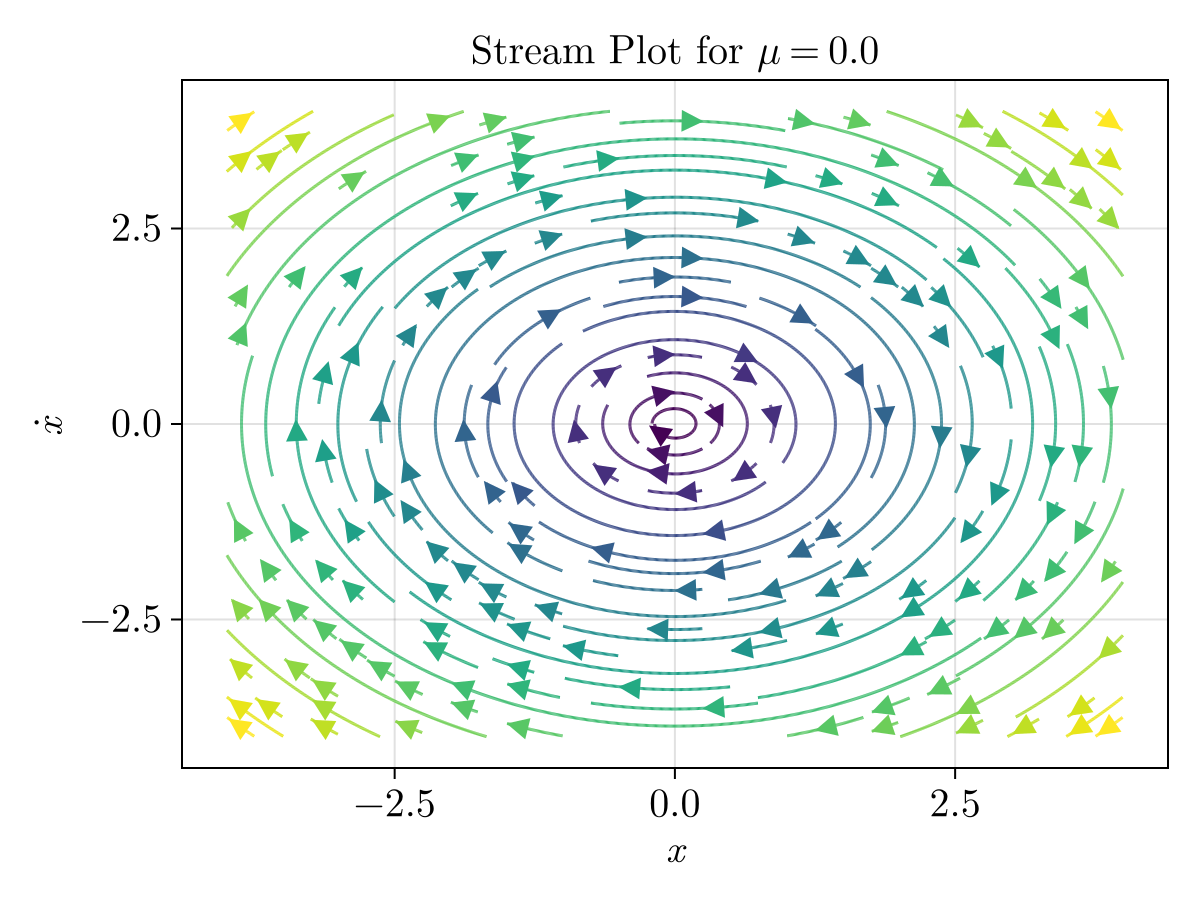
\includegraphics[width=\textwidth]{out/stream_01.png}

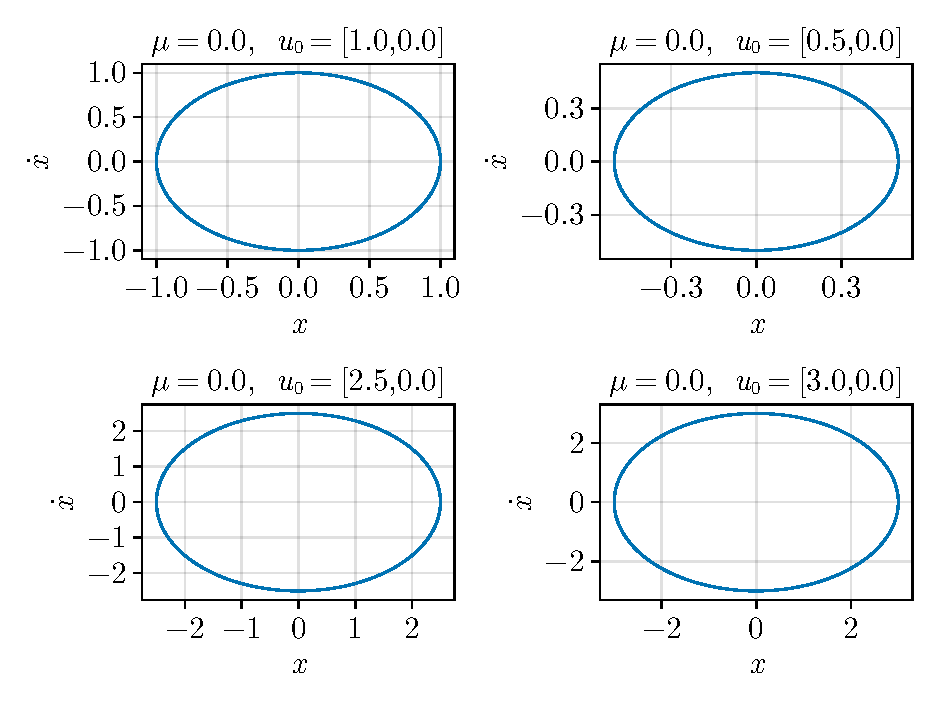
\includegraphics[width=\textwidth]{out/phase_01.pdf}

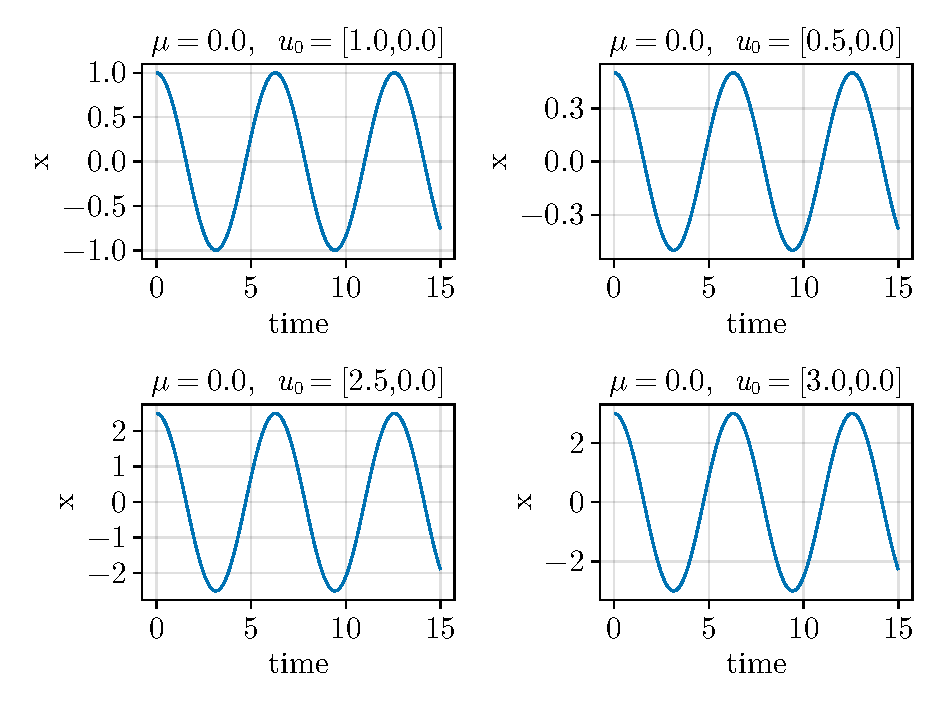
\includegraphics[width=\textwidth]{out/xfromt_01.pdf}

\clearpage

%
%
% plots for mu = 0.03125
%%%%%%%%%%%%%%%%%%
\subsection{Przypadek $\mu = 0.03125$}
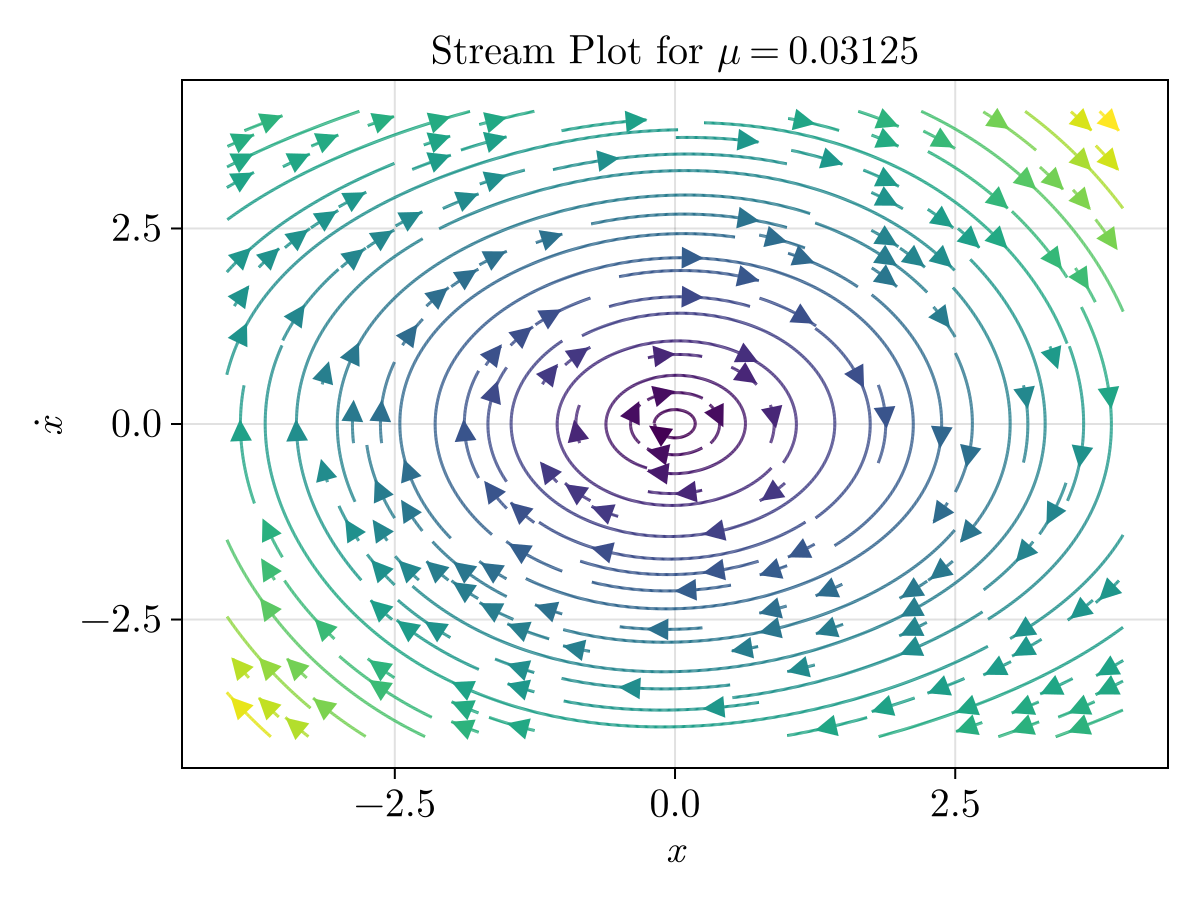
\includegraphics[width=\textwidth]{out/stream_02.png}

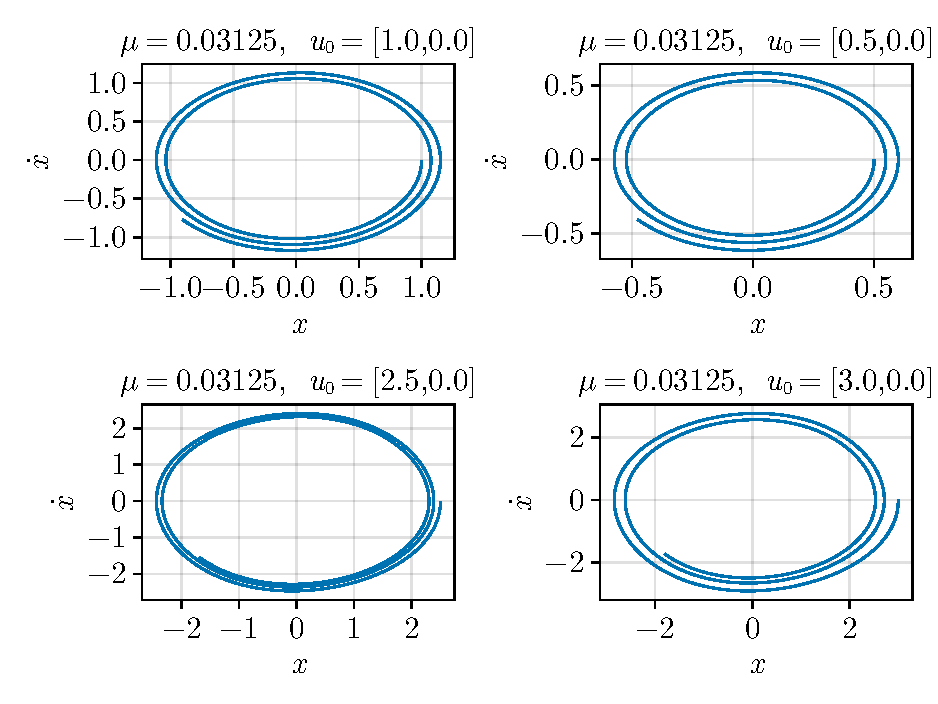
\includegraphics[width=\textwidth]{out/phase_02.pdf}

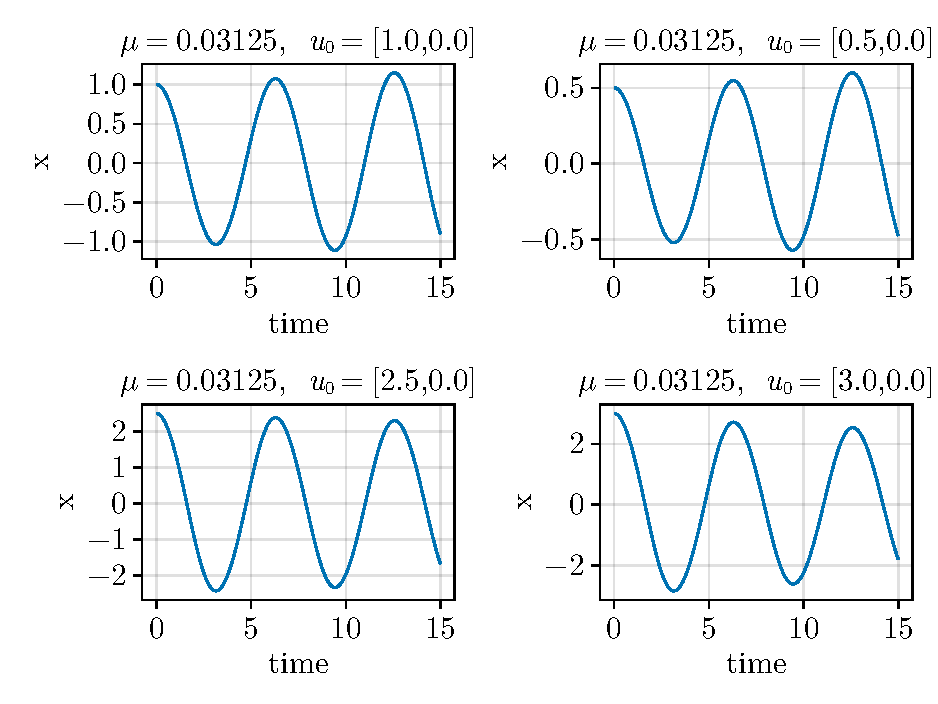
\includegraphics[width=\textwidth]{out/xfromt_02.pdf}

\clearpage

%
%
% plots for mu = 0.0625
%%%%%%%%%%%%%%%%%%
\subsection{Przypadek $\mu = 0.0625$}
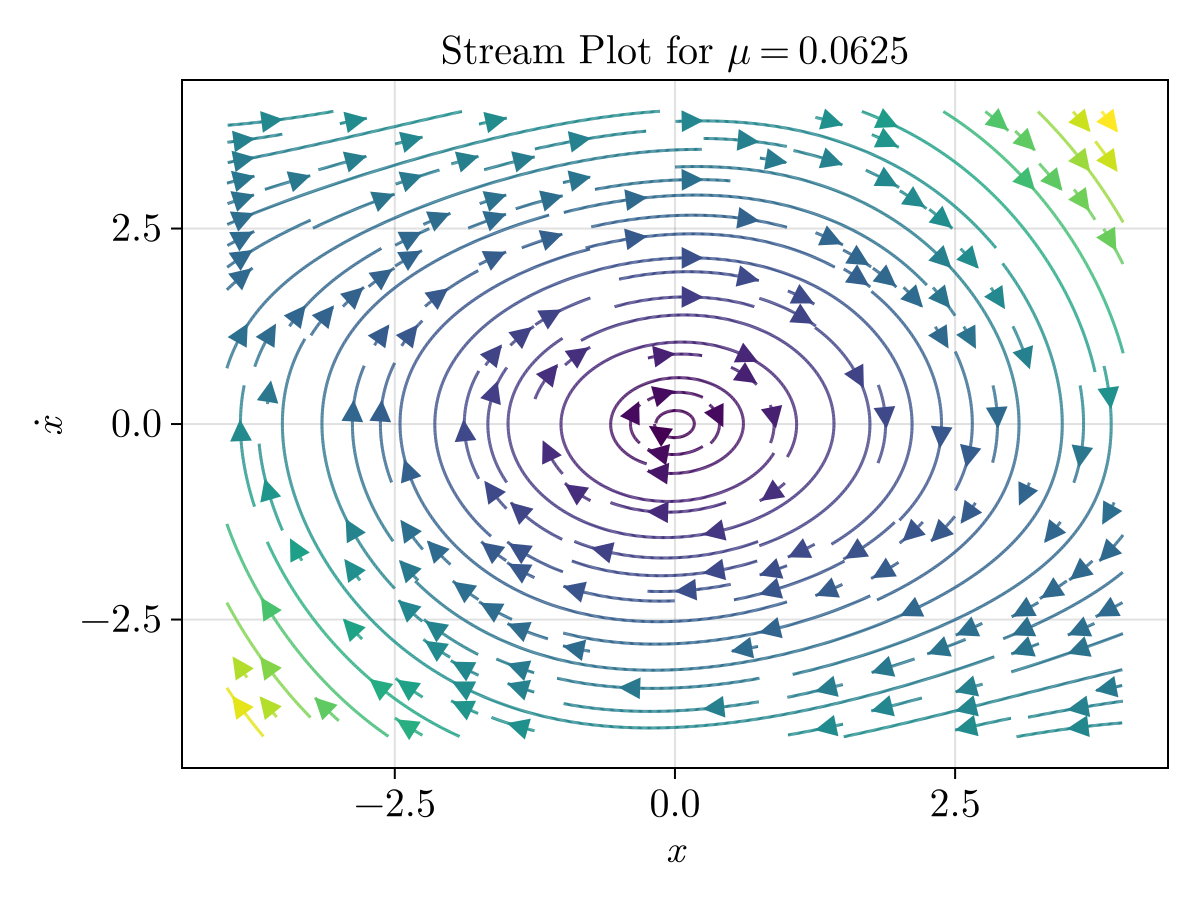
\includegraphics[width=\textwidth]{out/stream_03.png}

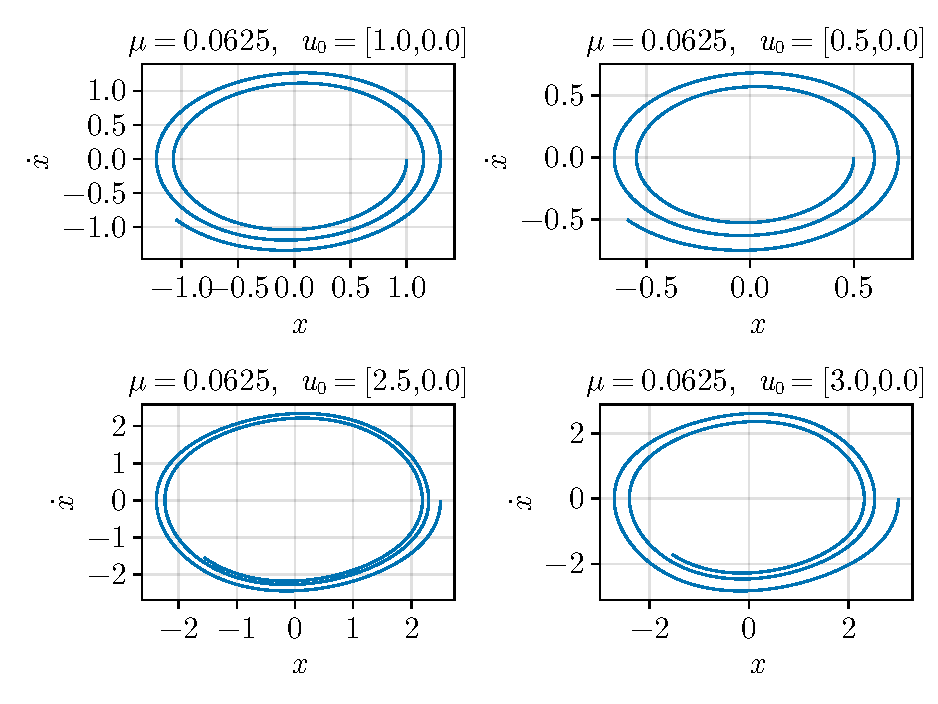
\includegraphics[width=\textwidth]{out/phase_03.pdf}

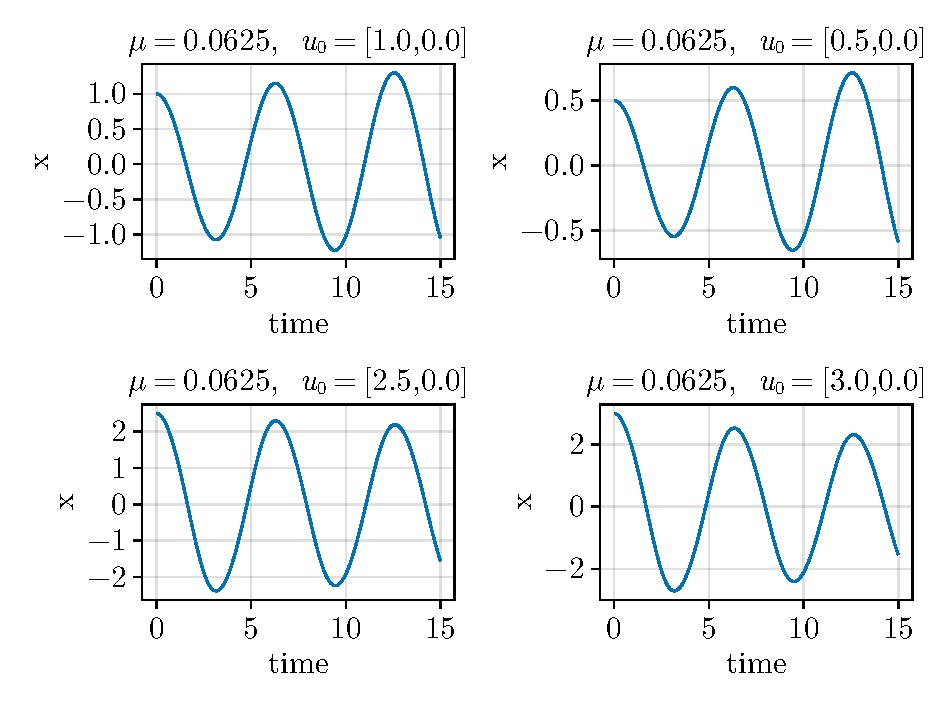
\includegraphics[width=\textwidth]{out/xfromt_03.pdf}

\clearpage

%
%
% plots for mu = 0.125
%%%%%%%%%%%%%%%%%%
\subsection{Przypadek $\mu = 0.125$}
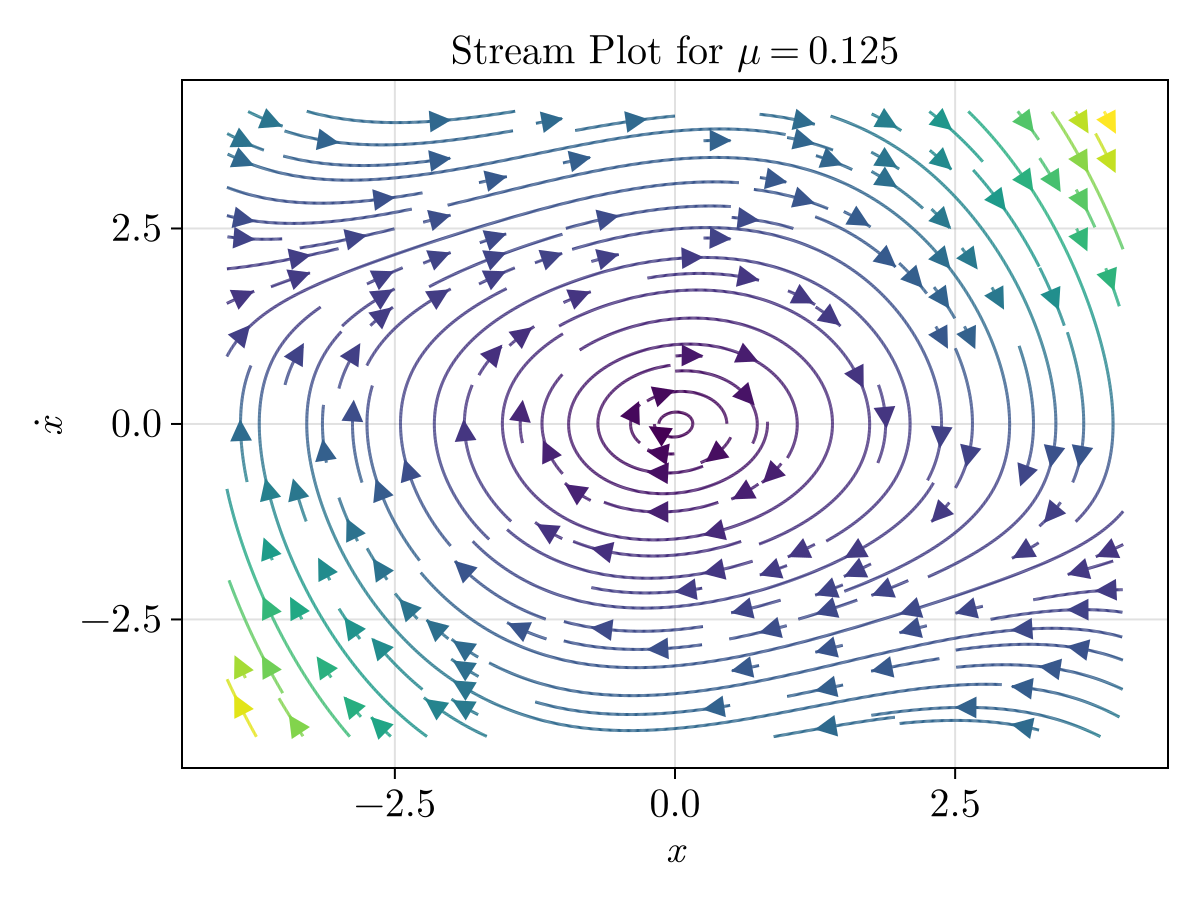
\includegraphics[width=\textwidth]{out/stream_04.png}

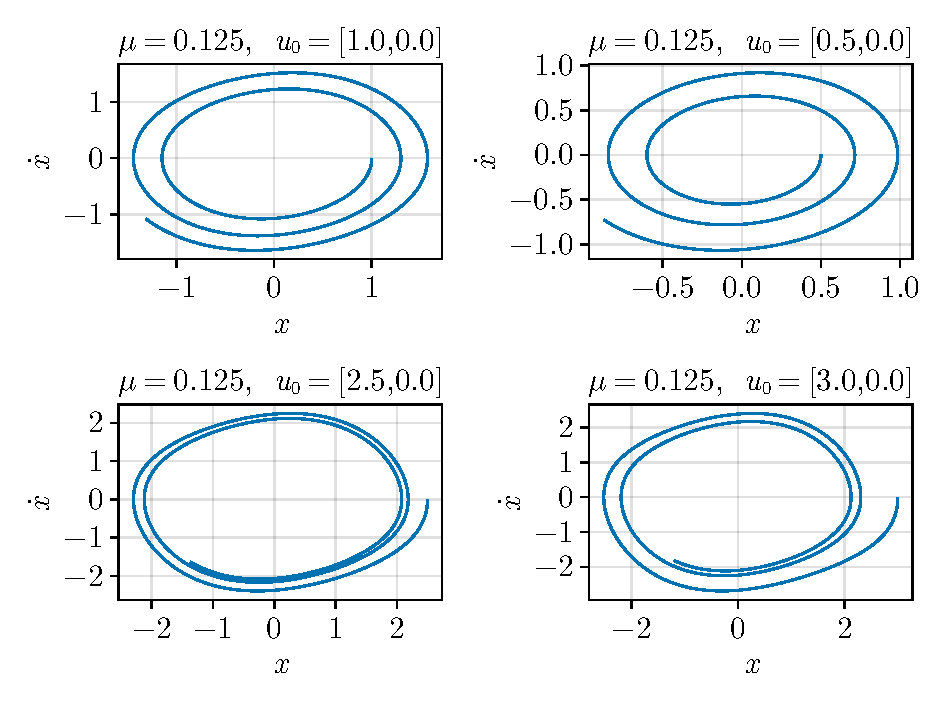
\includegraphics[width=\textwidth]{out/phase_04.pdf}

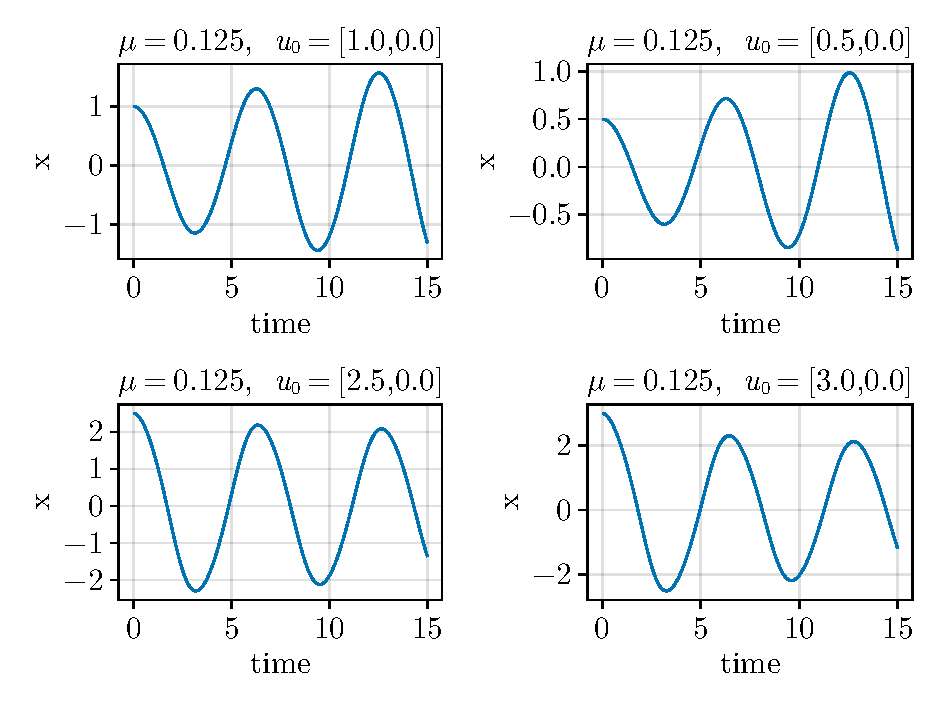
\includegraphics[width=\textwidth]{out/xfromt_04.pdf}

\clearpage

%
%
% plots for mu = 0.25
%%%%%%%%%%%%%%%%%%
\subsection{Przypadek $\mu = 0.25$}
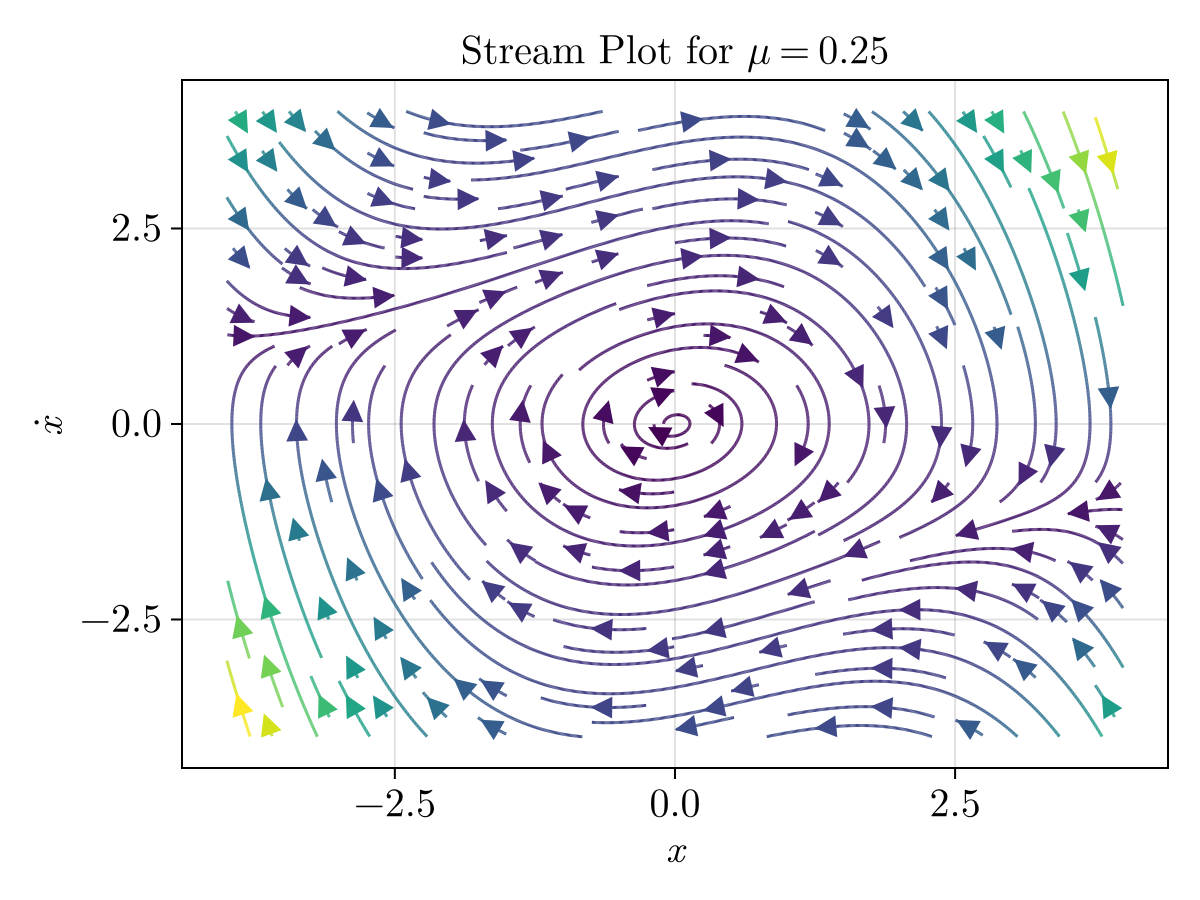
\includegraphics[width=\textwidth]{out/stream_05.png}

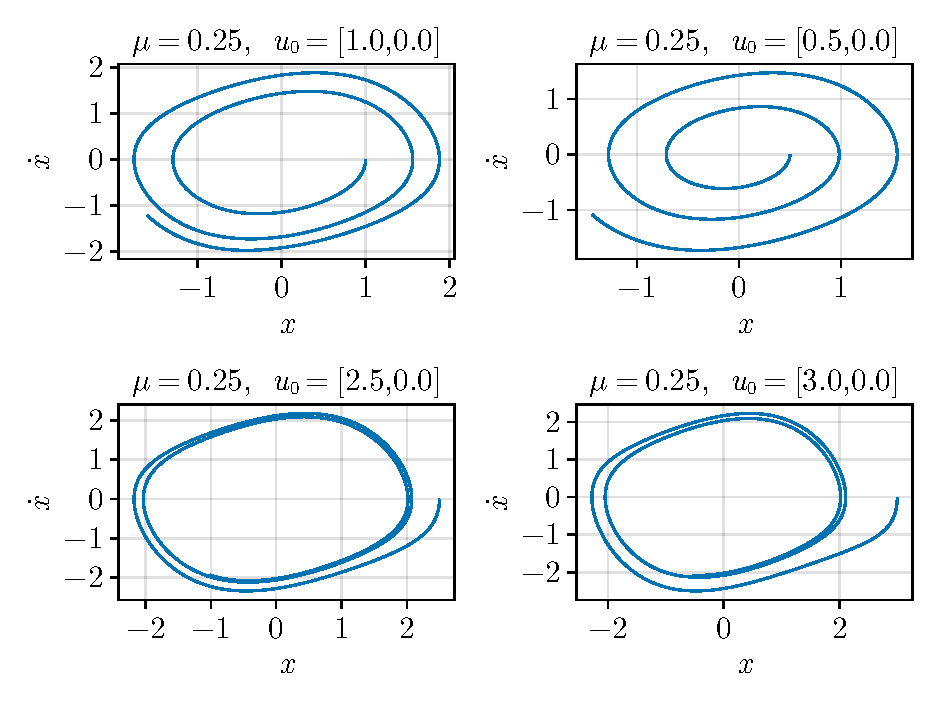
\includegraphics[width=\textwidth]{out/phase_05.pdf}

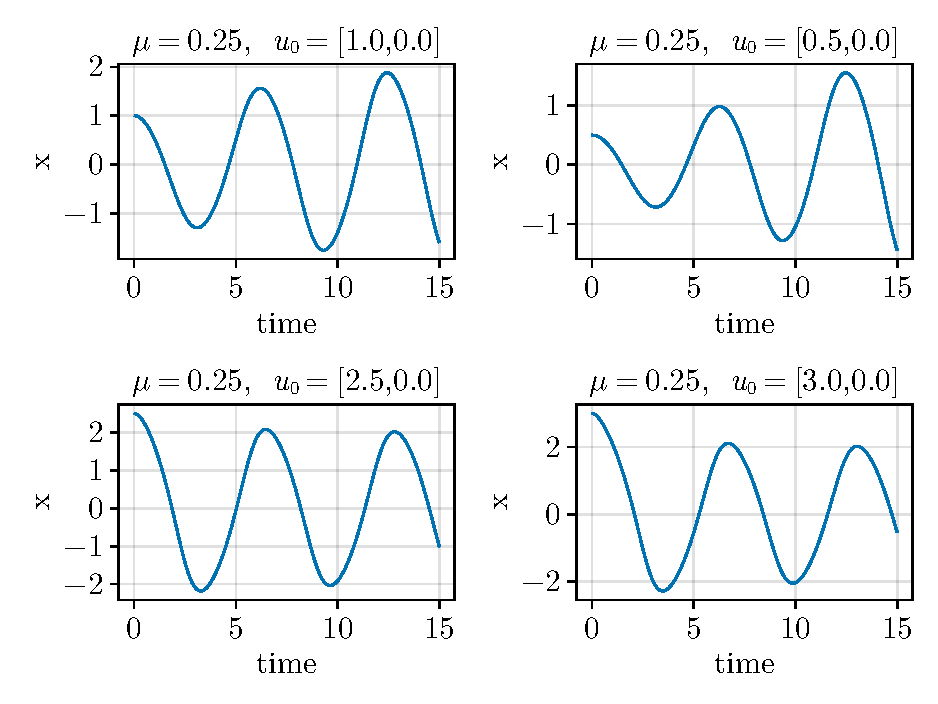
\includegraphics[width=\textwidth]{out/xfromt_05.pdf}

\clearpage

%
%
% plots for mu = 0.5
%%%%%%%%%%%%%%%%%%
\subsection{Przypadek $\mu = 0.5$}
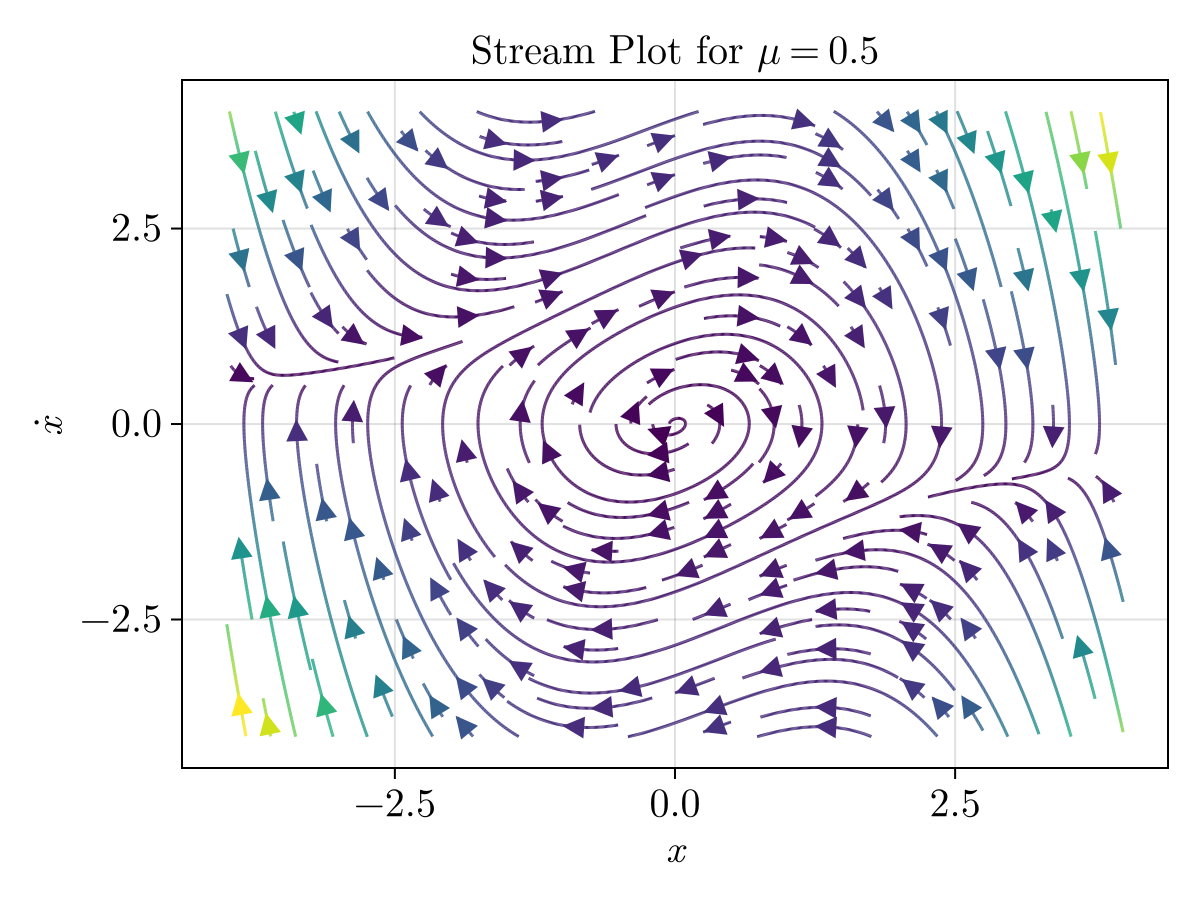
\includegraphics[width=\textwidth]{out/stream_06.png}

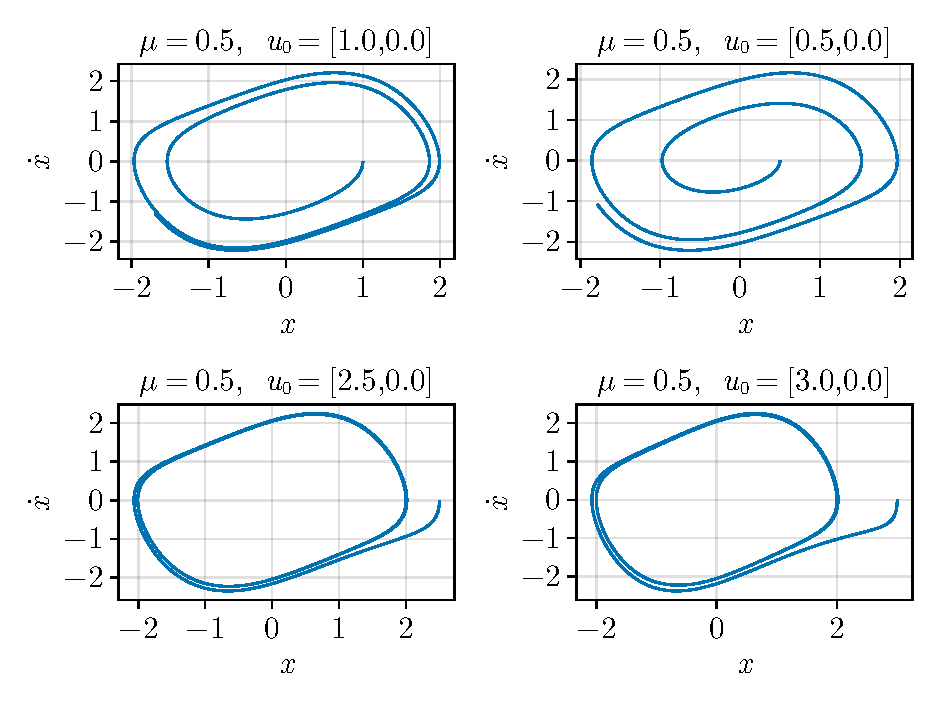
\includegraphics[width=\textwidth]{out/phase_06.pdf}

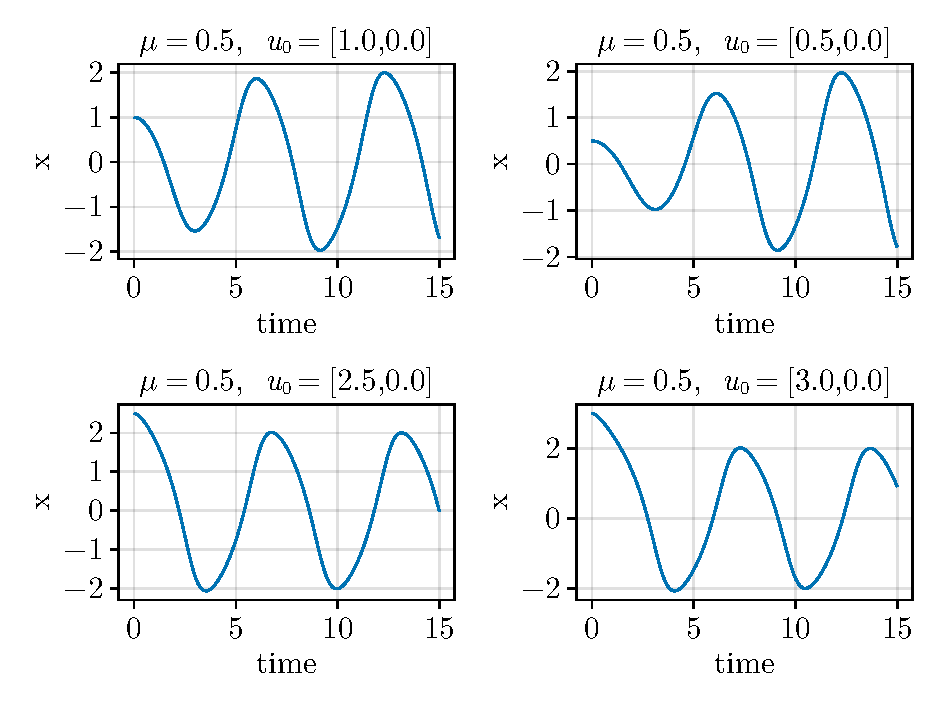
\includegraphics[width=\textwidth]{out/xfromt_06.pdf}

\clearpage

%
%
% plots for mu = 1.0
%%%%%%%%%%%%%%%%%%
\subsection{Przypadek $\mu = 1.0$}
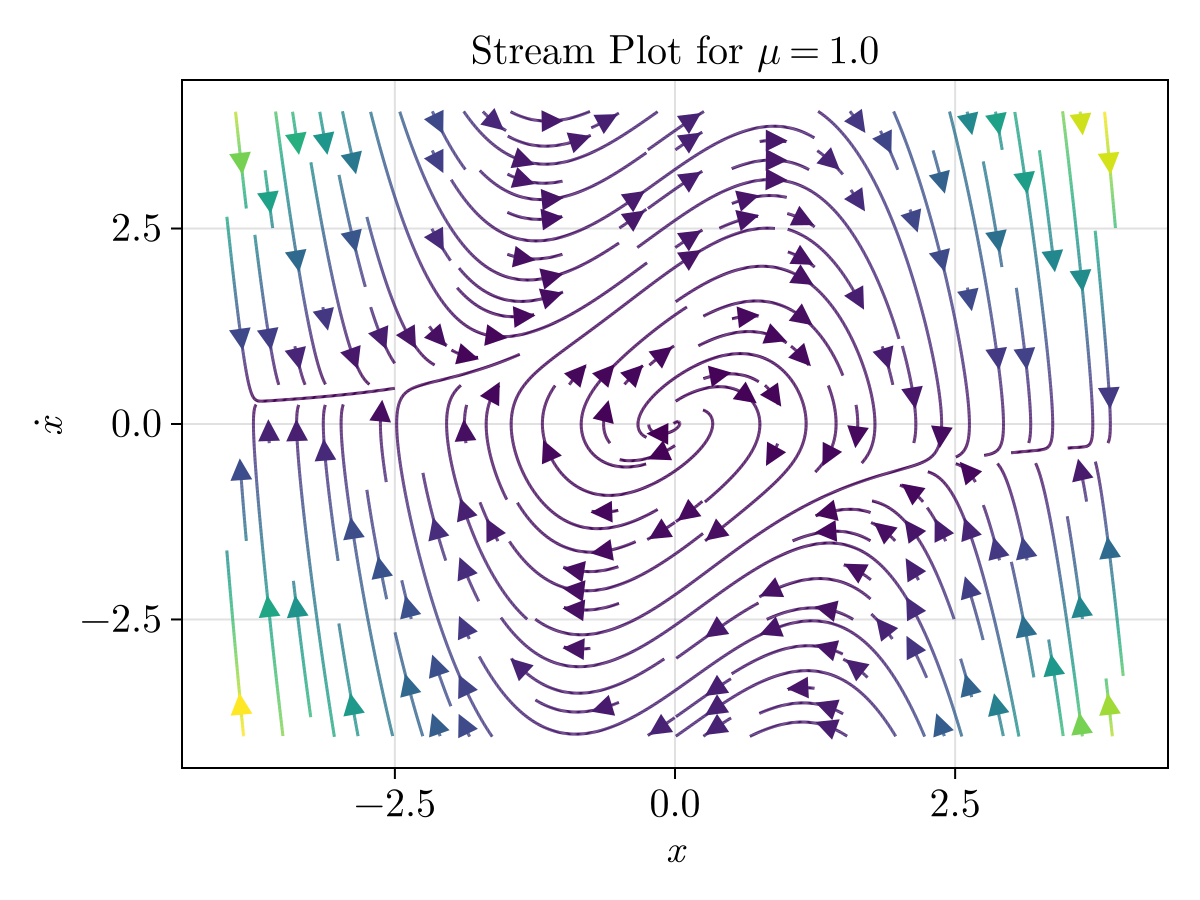
\includegraphics[width=\textwidth]{out/stream_07.png}

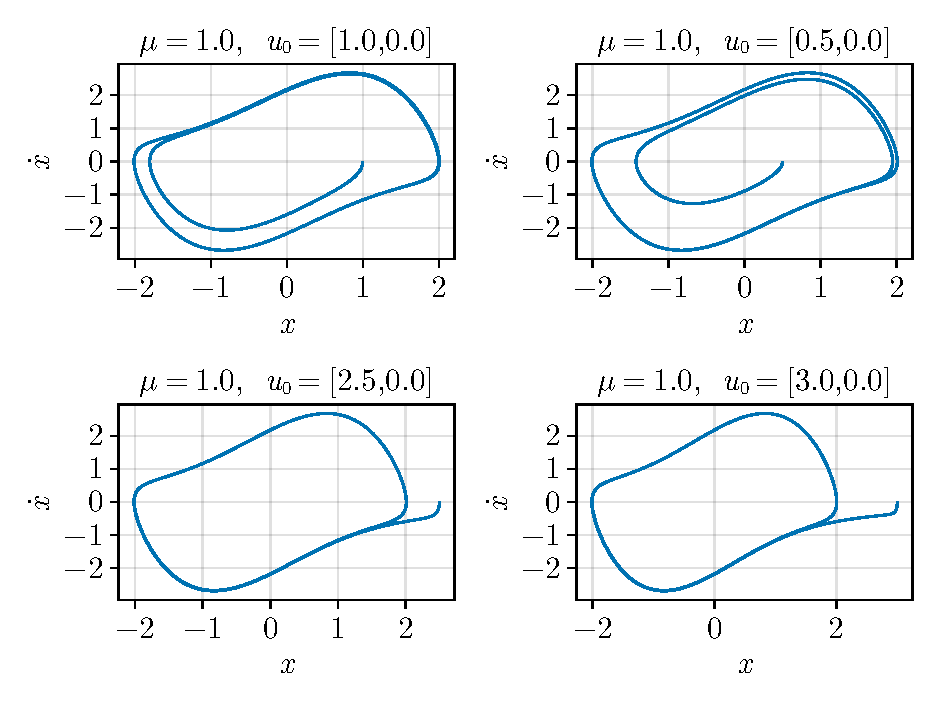
\includegraphics[width=\textwidth]{out/phase_07.pdf}

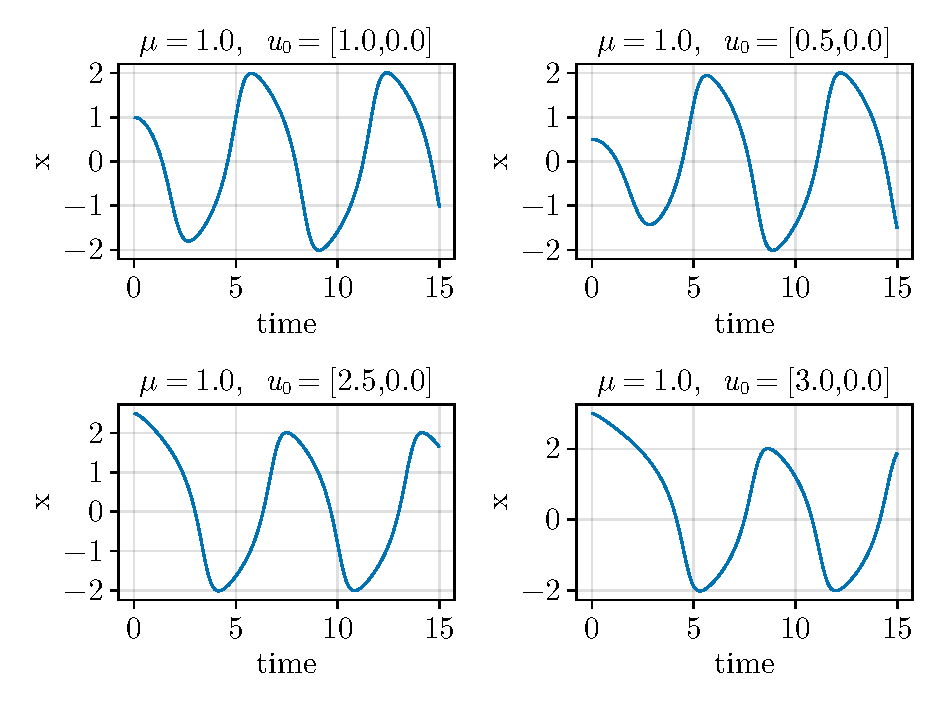
\includegraphics[width=\textwidth]{out/xfromt_07.pdf}

\clearpage

%
%
% plots for mu = 1.5
%%%%%%%%%%%%%%%%%%
\subsection{Przypadek $\mu = 1.5$}
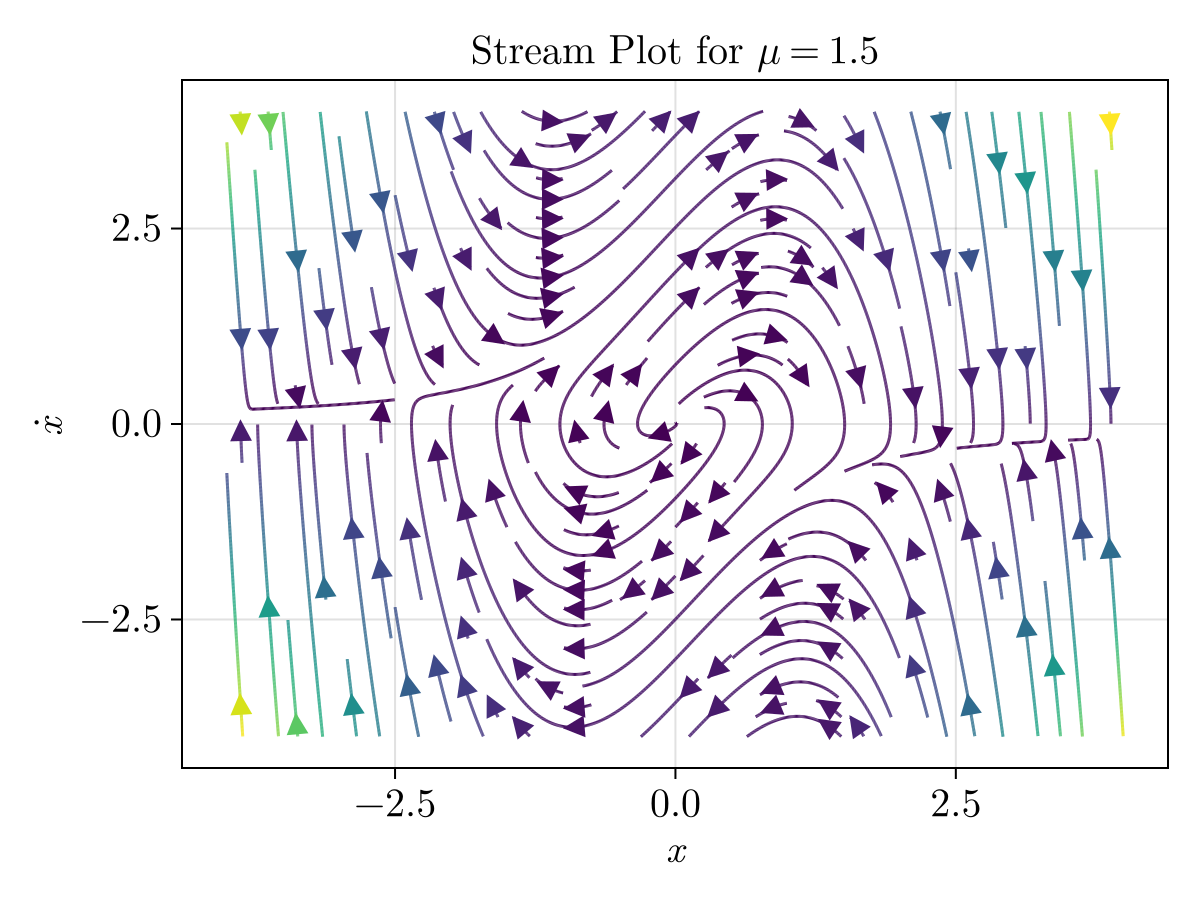
\includegraphics[width=\textwidth]{out/stream_08.png}

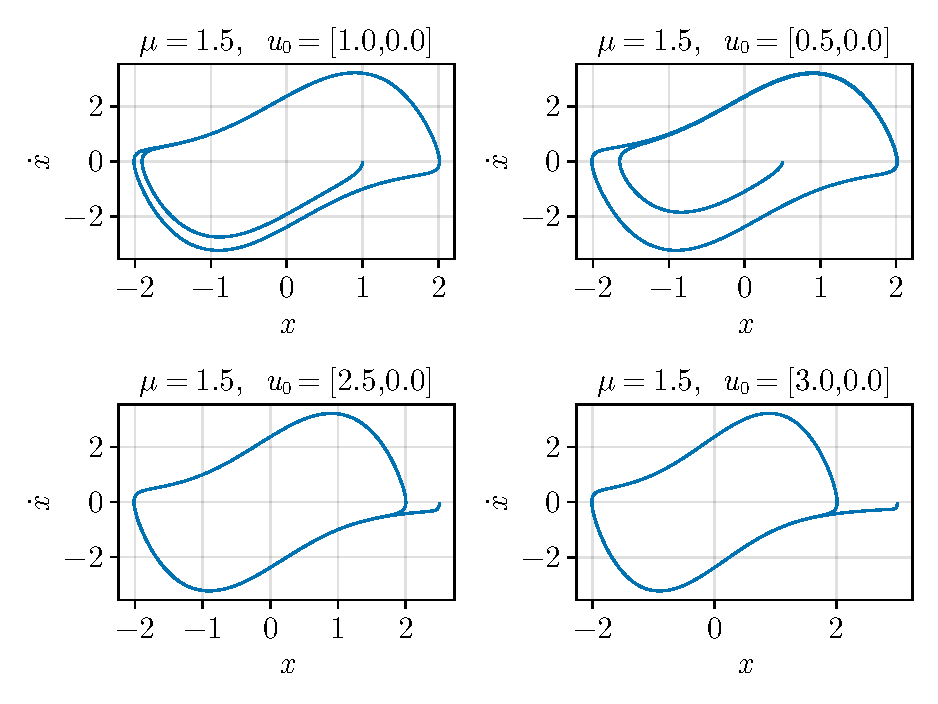
\includegraphics[width=\textwidth]{out/phase_08.pdf}

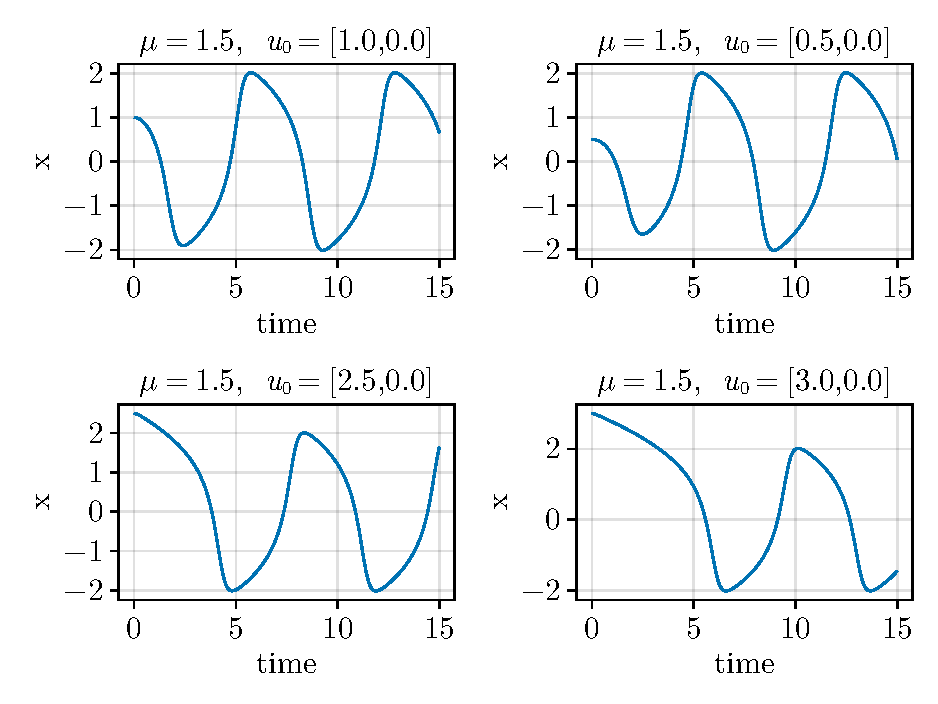
\includegraphics[width=\textwidth]{out/xfromt_08.pdf}

\clearpage

%
%
% plots for mu = 2.0
%%%%%%%%%%%%%%%%%%
\subsection{Przypadek $\mu = 2.0$}
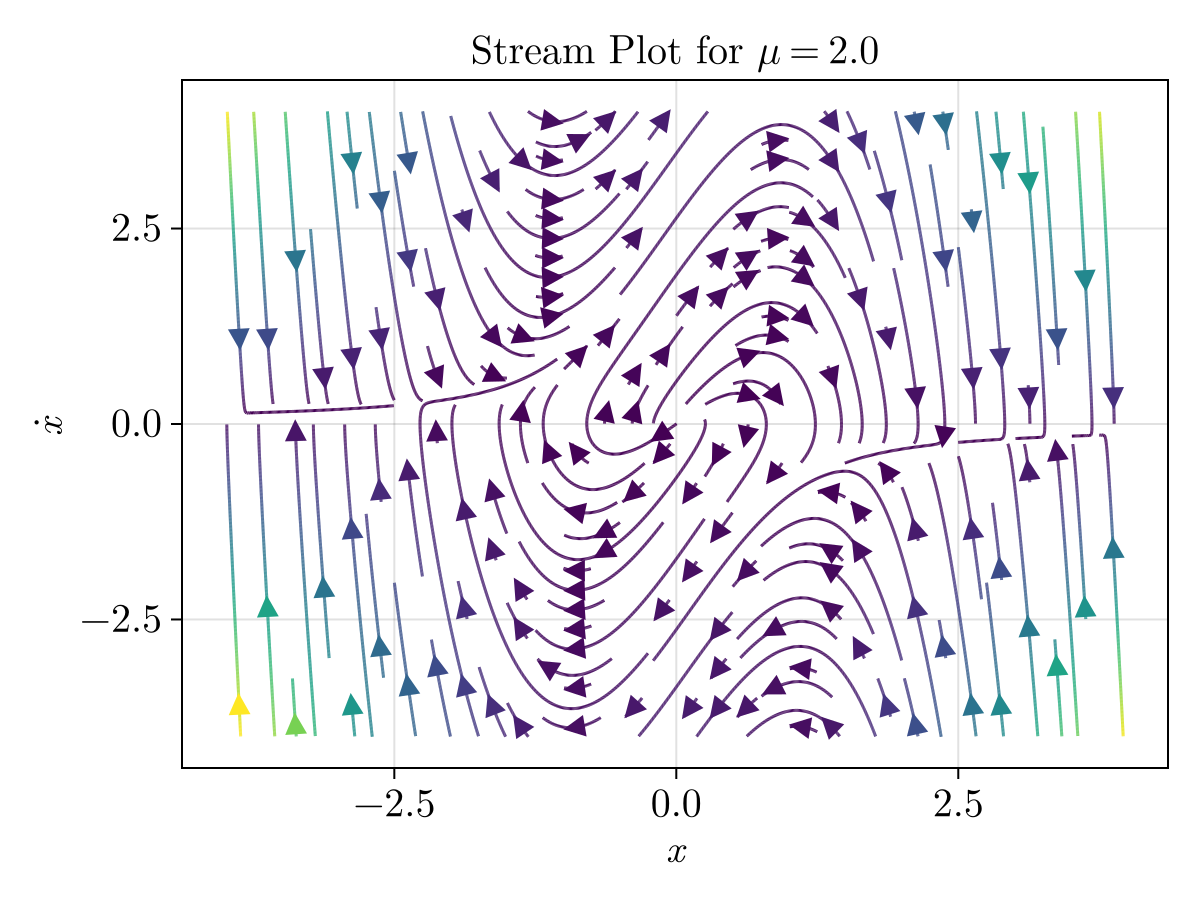
\includegraphics[width=\textwidth]{out/stream_09.png}

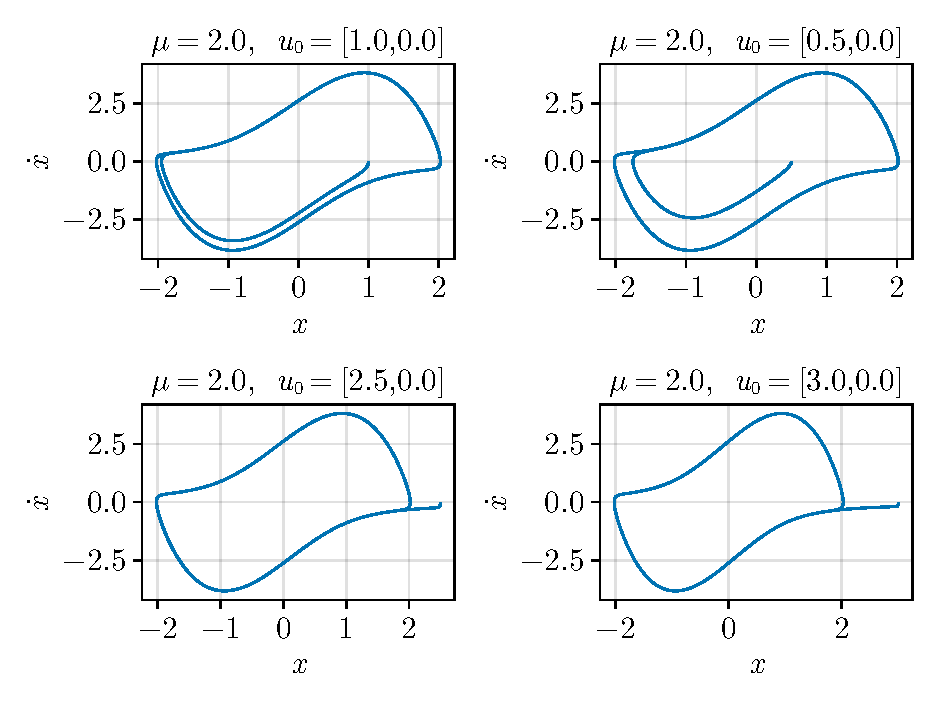
\includegraphics[width=\textwidth]{out/phase_09.pdf}

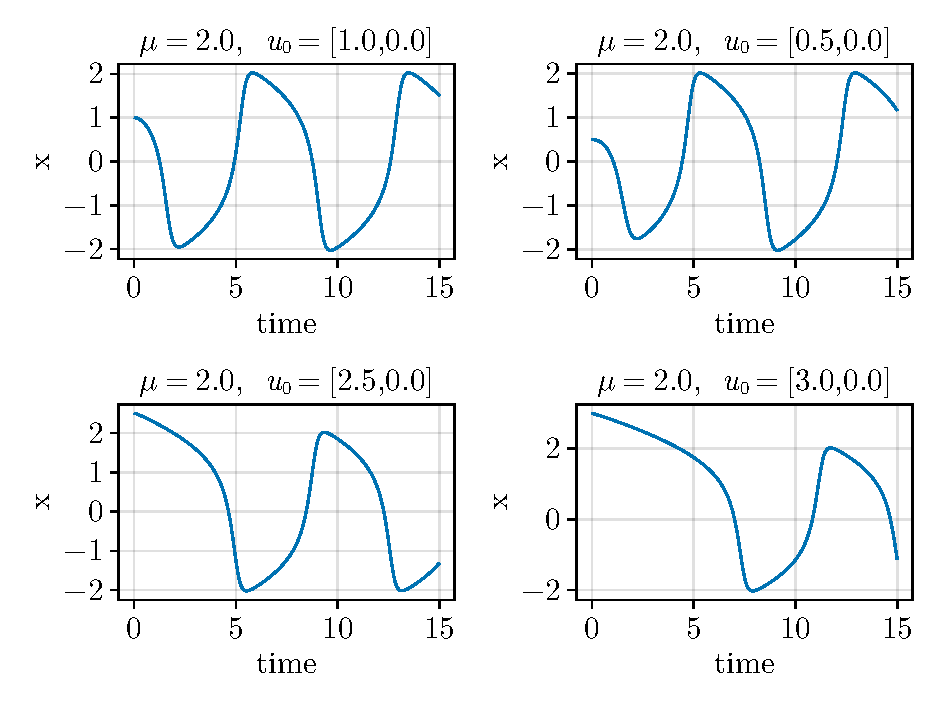
\includegraphics[width=\textwidth]{out/xfromt_09.pdf}

\clearpage

%
%
% plots for mu = 3.0
%%%%%%%%%%%%%%%%%%
\subsection{Przypadek $\mu = 3.0$}
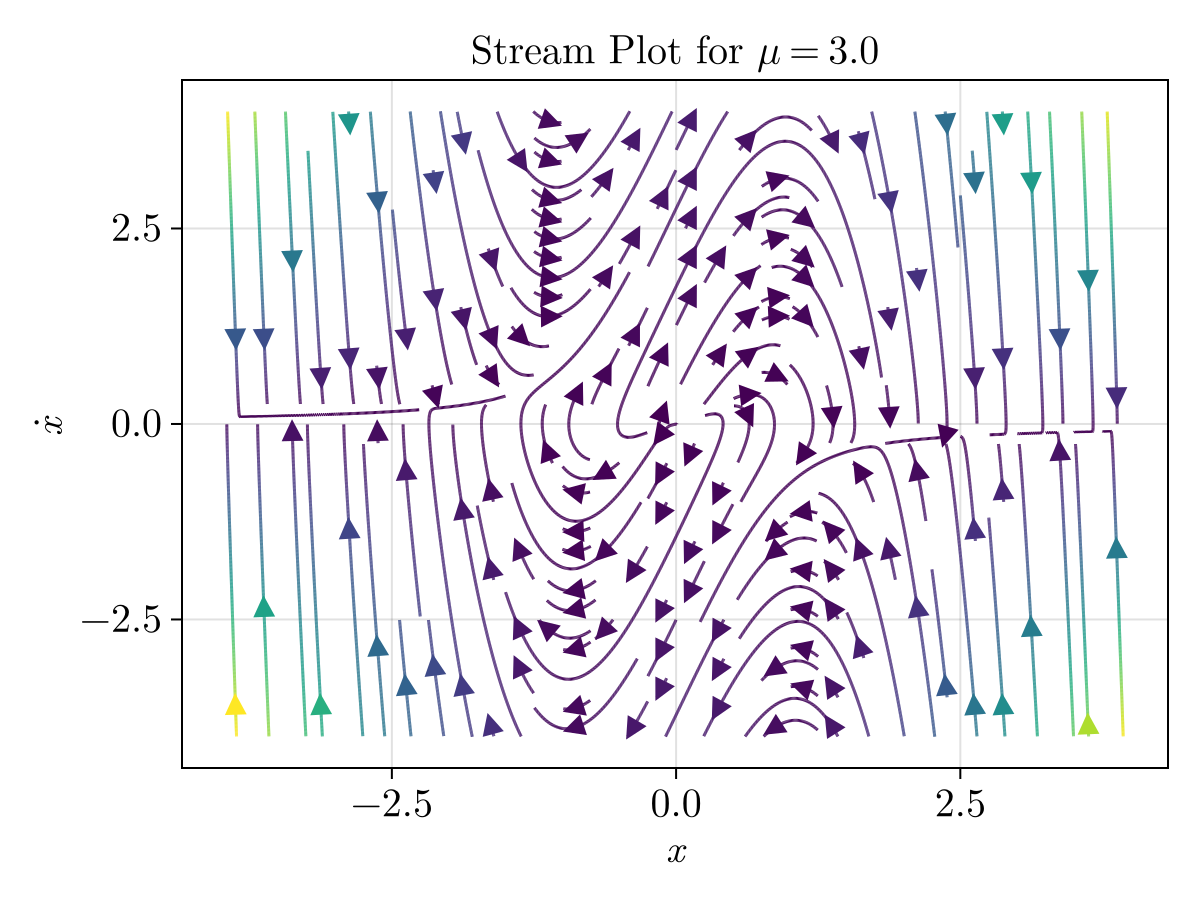
\includegraphics[width=\textwidth]{out/stream_10.png}

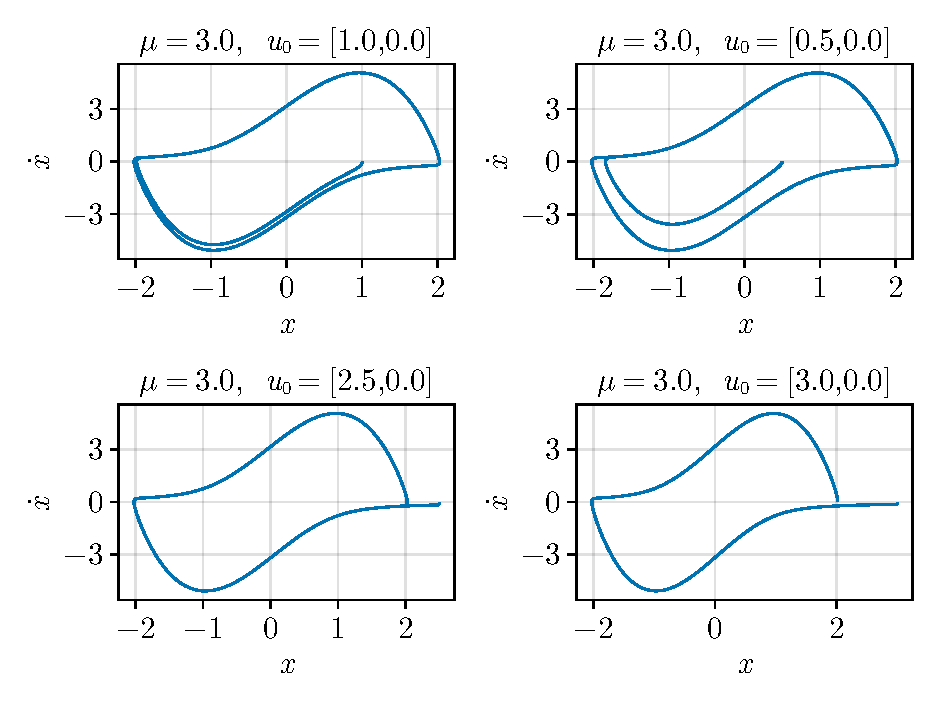
\includegraphics[width=\textwidth]{out/phase_10.pdf}

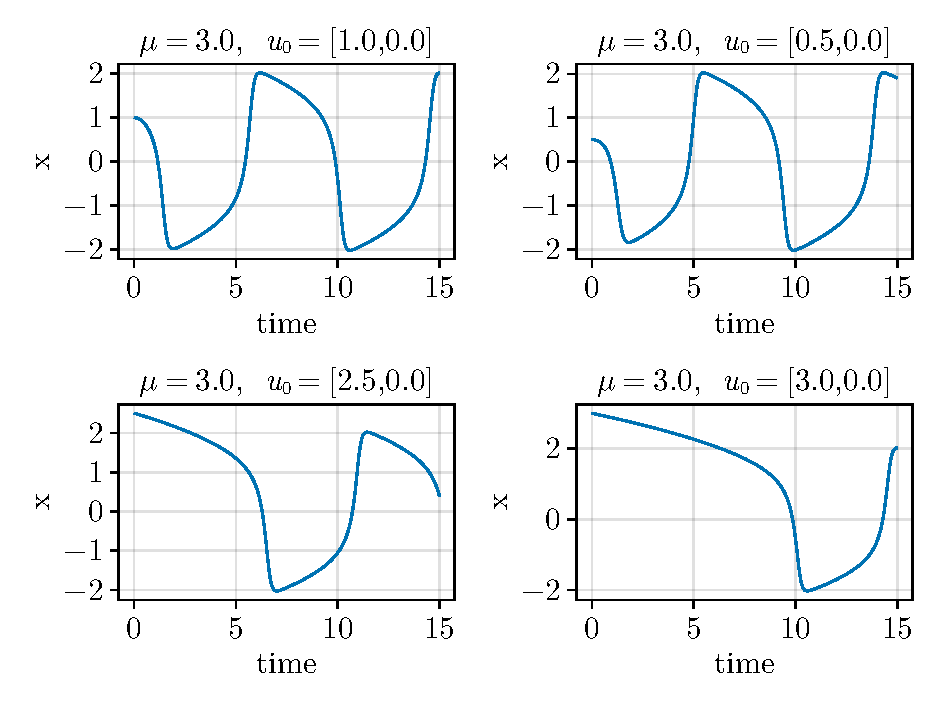
\includegraphics[width=\textwidth]{out/xfromt_10.pdf}

\clearpage

%
%
% plots for mu = 5.0
%%%%%%%%%%%%%%%%%%
\subsection{Przypadek $\mu = 5.0$}
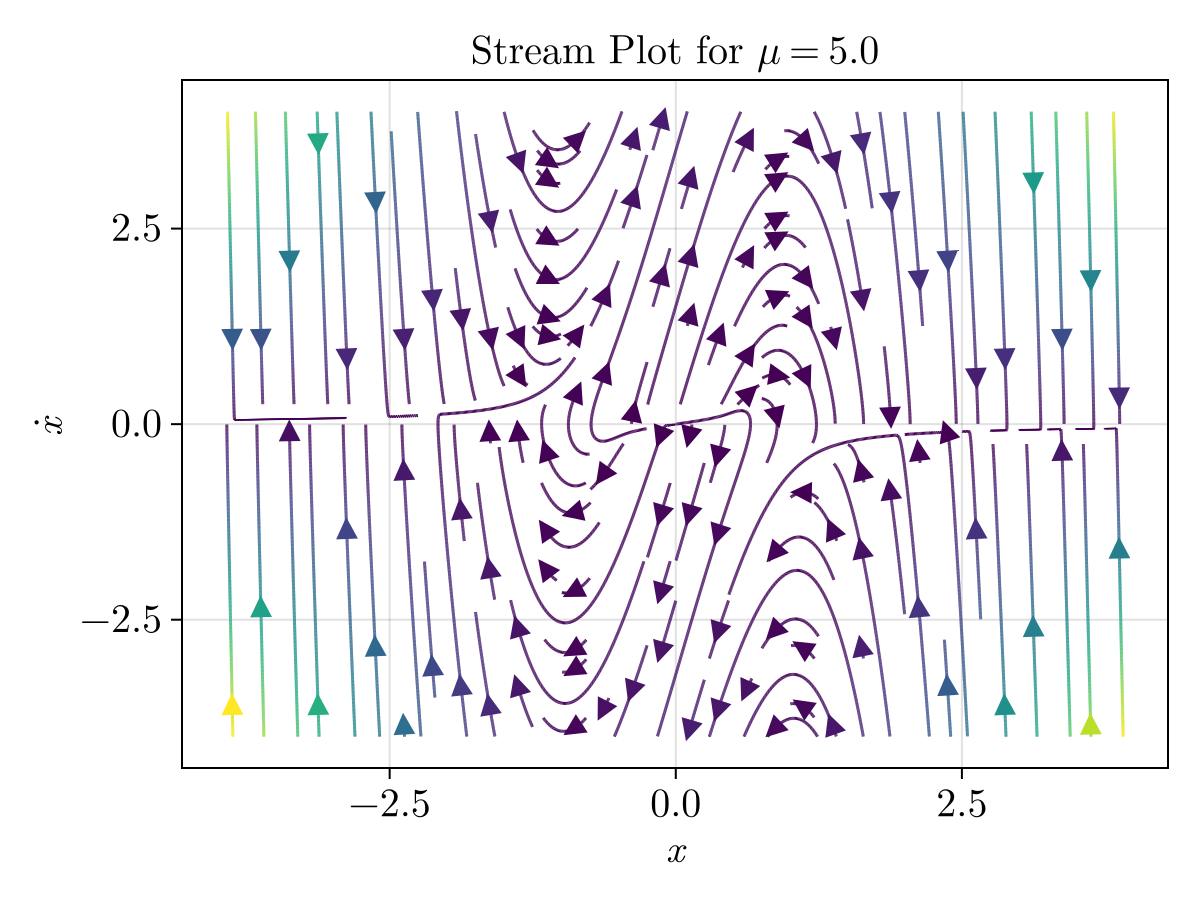
\includegraphics[width=\textwidth]{out/stream_11.png}

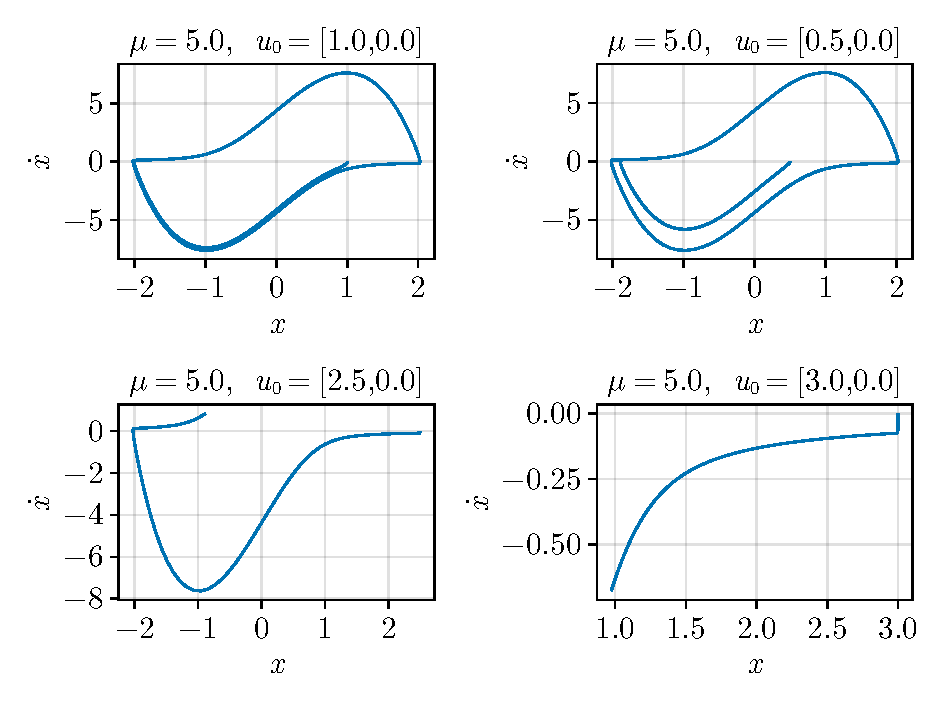
\includegraphics[width=\textwidth]{out/phase_11.pdf}

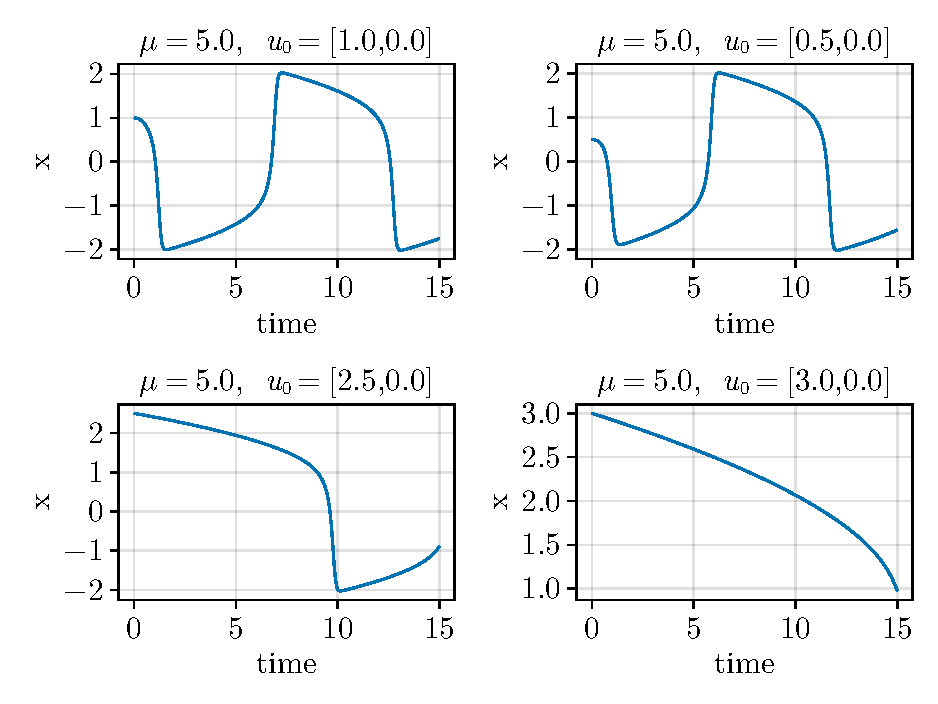
\includegraphics[width=\textwidth]{out/xfromt_11.pdf}

\clearpage

%
%
% plots for mu = 7.0
%%%%%%%%%%%%%%%%%%
\subsection{Przypadek $\mu = 7.0$}
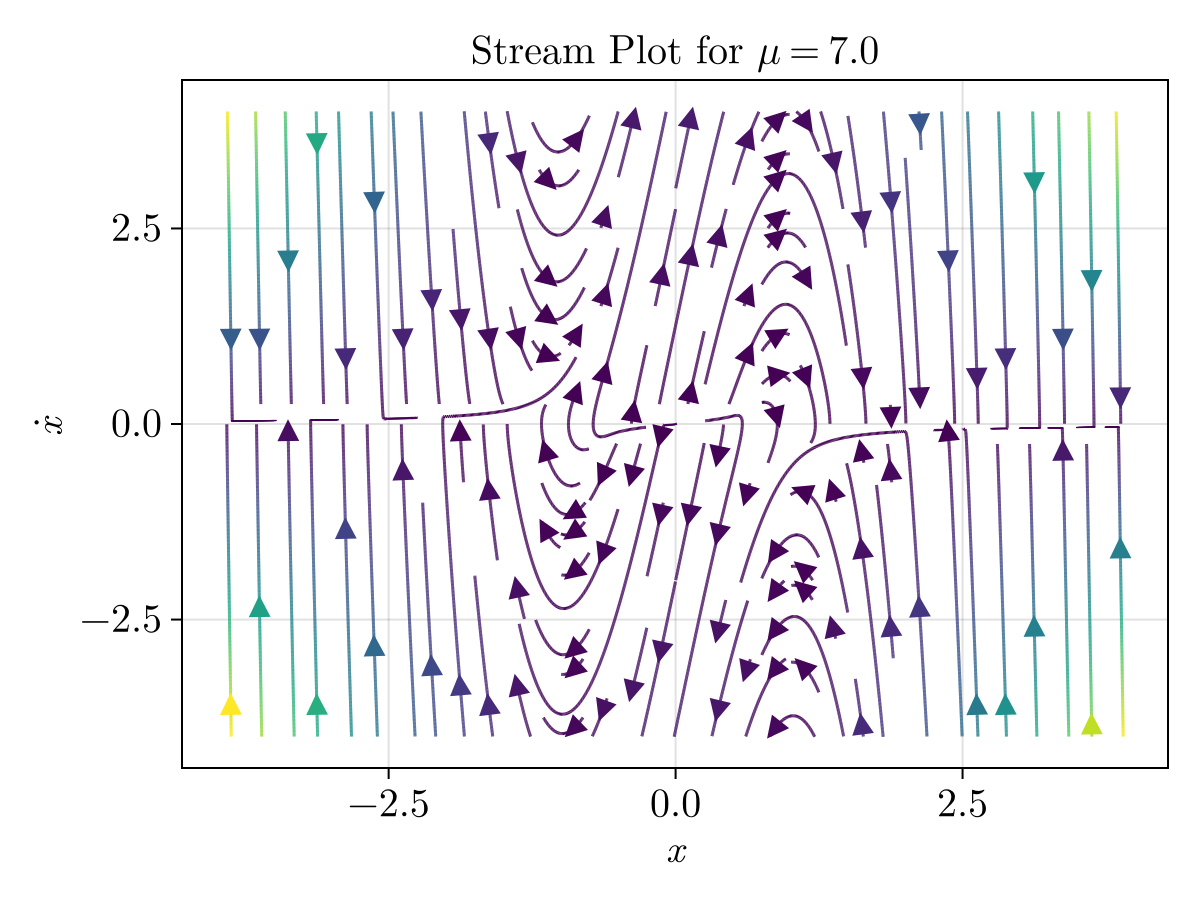
\includegraphics[width=\textwidth]{out/stream_12.png}

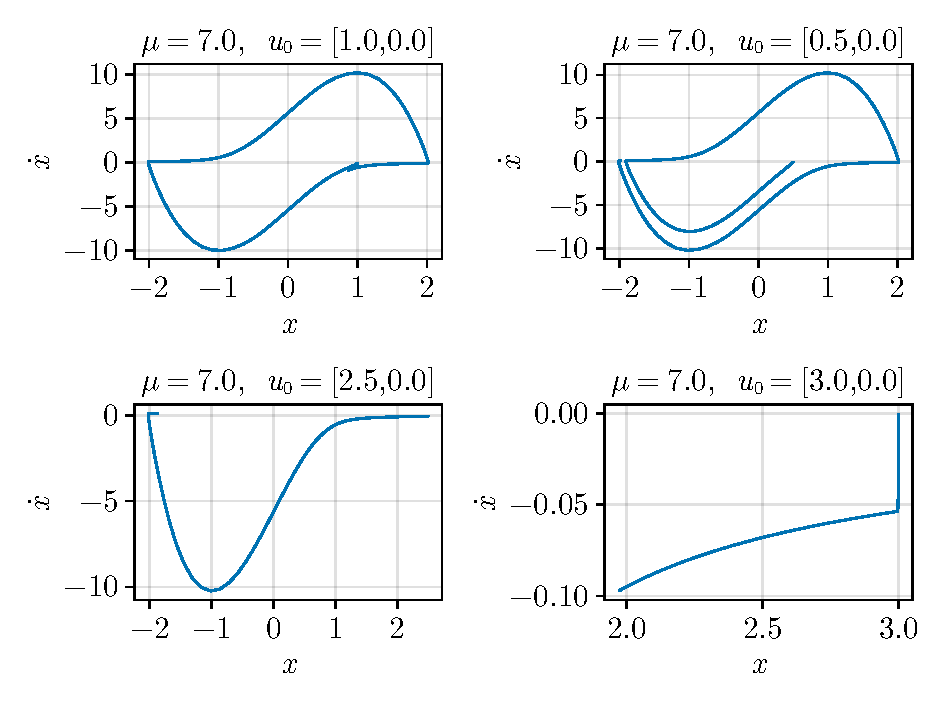
\includegraphics[width=\textwidth]{out/phase_12.pdf}

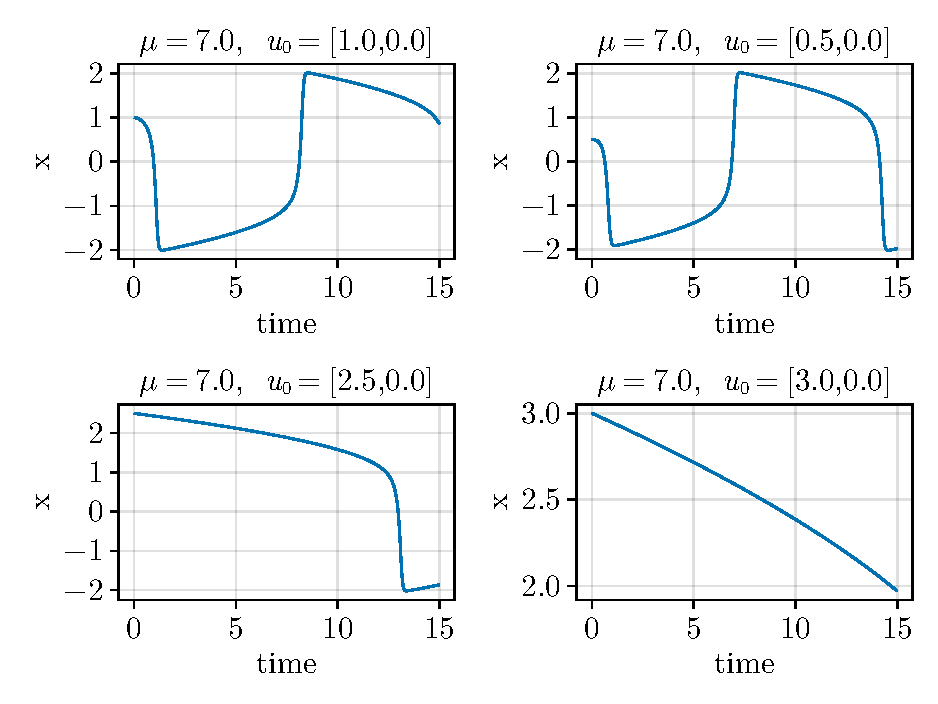
\includegraphics[width=\textwidth]{out/xfromt_12.pdf}

\clearpage

%
%
% plots for mu = 9.0
%%%%%%%%%%%%%%%%%%
\subsection{Przypadek $\mu = 9.0$}
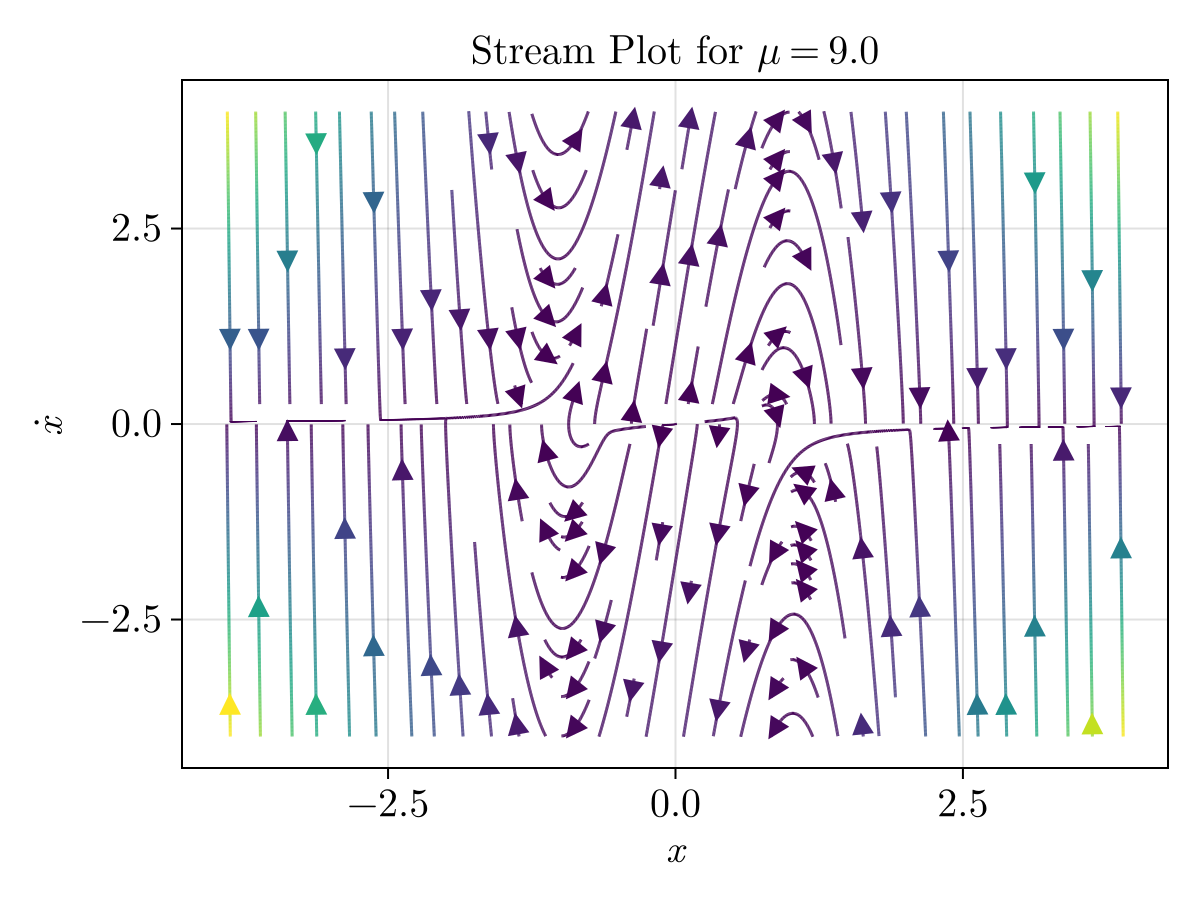
\includegraphics[width=\textwidth]{out/stream_13.png}

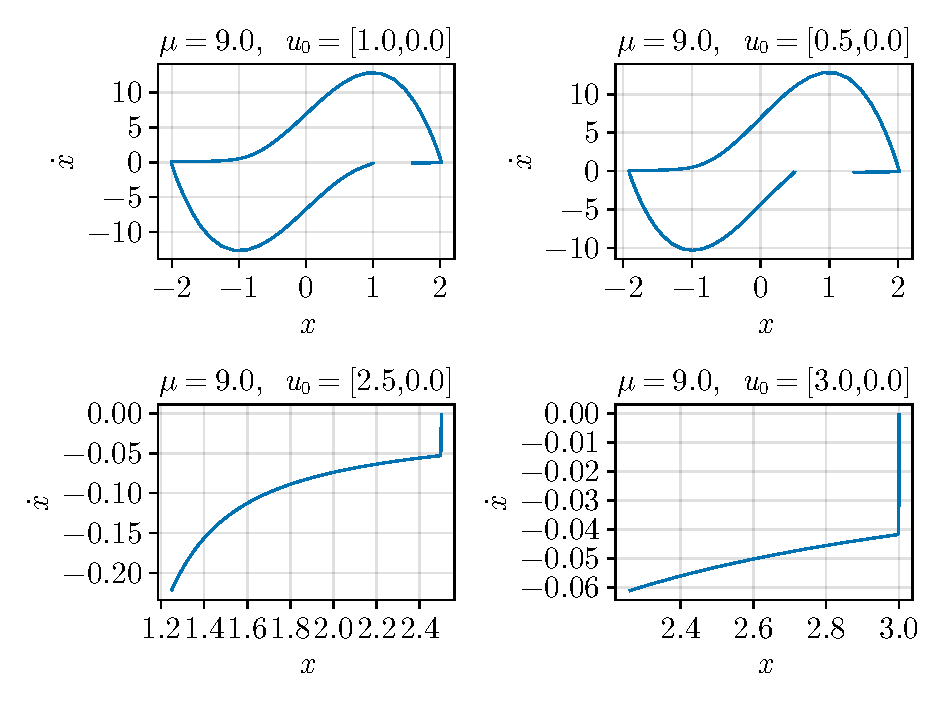
\includegraphics[width=\textwidth]{out/phase_13.pdf}

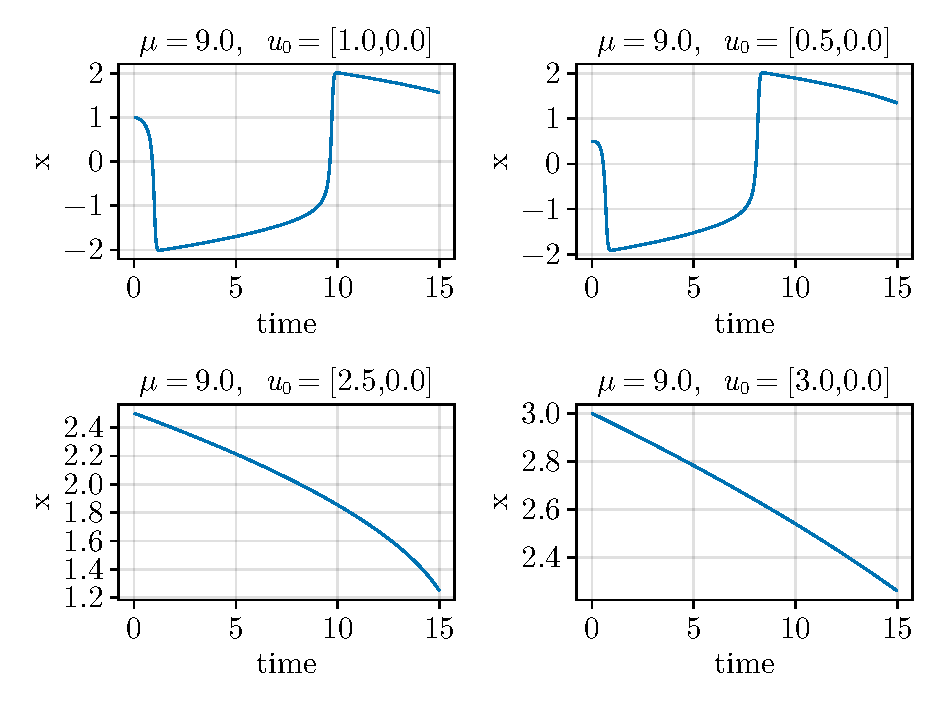
\includegraphics[width=\textwidth]{out/xfromt_13.pdf}

\clearpage




\end{document}